\section{Theoretical Background}
% \addcontentsline{toc}{section}{Theoretical Background}
\fancyhead[R]{Theoretical Background}

\subsection{Principles of Enzymology}
\label{sec:Principles of Enzymology}

Enzymology is the study of enzymes, which are biological catalysts that accelerate biochemical reactions in living organisms. These macromolecules are essential for various cellular processes, including metabolism, DNA replication, and signal transduction. The understanding of enzyme structure, function, and kinetics is crucial for developing applications in biotechnology, medicine, and environmental science. \autocite{robinsonEnzymesPrinciplesBiotechnological2015}

\subsubsection{Enzyme Classification and Function}
\label{sec:Enzyme Classification and Function}

Enzymes are classified based on the reactions they catalyze, following a system established by the Enzyme Commission (EC). This classification system groups enzymes into six main classes, each with specific types of reactions they facilitate:

\begin{compactenum}
    \item \textbf{Oxidoreductases:} These enzymes catalyze oxidation-reduction reactions, where the transfer of electrons occurs between molecules. Examples include dehydrogenases and oxidases.
    
    \item \textbf{Transferases:} These enzymes transfer functional groups from one molecule to another. Examples include kinases, which transfer phosphate groups.
    
    \item \textbf{Hydrolases:} These enzymes catalyze the hydrolysis of various bonds, including ester, glycosidic, peptide, and others. Examples include proteases and lipases.
    
    \item \textbf{Lyases:} These enzymes add or remove groups to form double bonds, without hydrolysis or oxidation. Examples include decarboxylases and dehydratases.
    
    \item \textbf{Isomerases:} These enzymes catalyze the rearrangement of atoms within a molecule, leading to isomerization. Examples include racemases and epimerases.
    
    \item \textbf{Ligases:} These enzymes catalyze the joining of two molecules with the simultaneous hydrolysis of a diphosphate bond in ATP or a similar triphosphate. Examples include synthetases and carboxylases.
    
\end{compactenum}

-- Überleitung finden --
The three-dimensional (3D) structure of enzymes is fundamental to their function. Enzymes are composed of one or more polypeptide chains that fold into specific shapes to form the active site. The active site is where substrate molecules bind and undergo a chemical reaction. The enzyme structure serves as a scaffold to support and correctly position the active site for optimal catalytic activity. 

\begin{figure}[hbt]
    \centering
    \begin{minipage}[t]{.9\textwidth}
    \caption{Organisation of enzyme structure and lysozyme example.}
    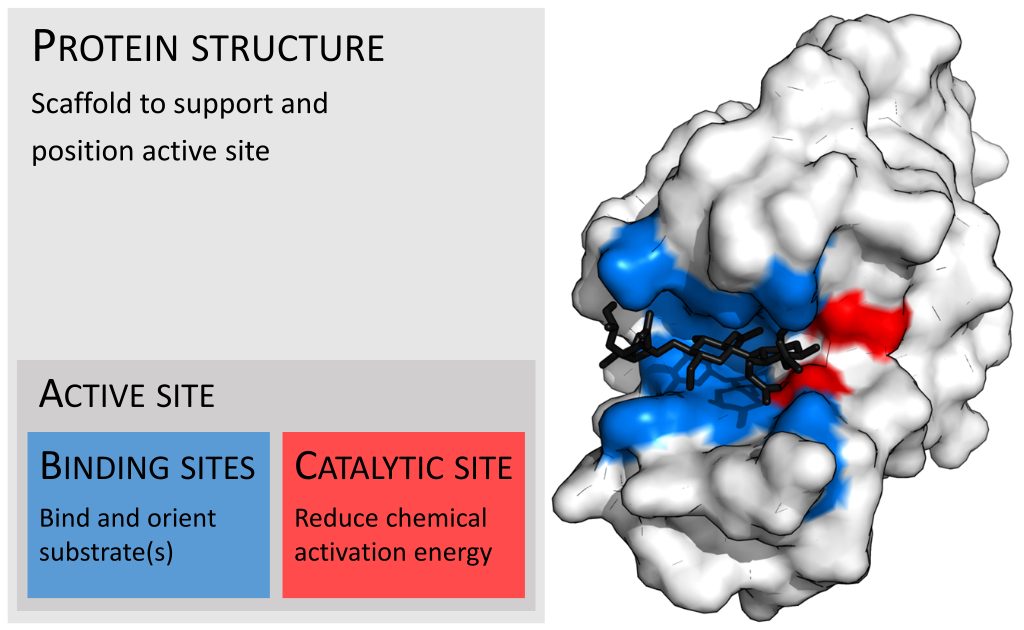
\includegraphics[width=1\textwidth]{img/EnzymeStructure.svg.png}\\
    \source{Thomas Shafee, CC BY 4.0 via Wikimedia Commons}
    \label{fig:EnzymeStructure}
    \end{minipage}
\end{figure}

\begin{itemize}
    \item \textbf{Protein Structure:} The overall structure of the enzyme provides the framework that supports and positions the active site. This structure is critical for the enzyme's stability and functionality. The enzyme's polypeptide chains fold into a unique 3D shape, creating a specific environment for the active site.
    \item \textbf{Active Site:} The active site includes two critical regions: binding sites and the catalytic site. The binding sites (highlighted in blue) are regions where substrates bind to the enzyme. These sites ensure that the substrates are properly oriented for the reaction. The catalytic site (highlighted in red) is the region where the chemical reaction occurs. The catalytic site often contains amino acids with specific functional groups that participate directly in the reaction, reducing the activation energy required for the reaction to proceed.
\end{itemize}

The precise arrangement of amino acids in the active site allows enzymes to be highly specific for their substrates, facilitating efficient catalysis. This specificity is a key feature that enables enzymes to perform their roles in various biochemical pathways with high precision.

A study by Veselovsky et al. (2001) emphasizes the importance of visualizing active site structures, even for enzymes with unknown 3D structures. By analyzing enzyme interactions with reversible competitive inhibitors and molding the substrate-binding region, researchers can predict the shape and dimensions of the active site. This approach has been validated by comparing it with known enzyme-inhibitor complexes, demonstrating its utility in understanding enzyme function and aiding in the search for new ligands.\autocite{veselovskyApproachVisualizationActive2001}

\subsubsection{Role of Enzymes in Biodegradation}
\label{sec:Role of Enzymes in Biodegradation}

Enzymes play a crucial role in the biodegradation of pollutants, including pesticides. The process involves the breakdown of complex organic molecules into simpler, less toxic forms. This degradation is essential for reducing environmental pollution and mitigating the adverse effects of hazardous chemicals.

Hydrolytic Enzymes: Hydrolytic enzymes, such as esterases and amidases, catalyze the cleavage of ester and amide bonds in pesticide molecules. This hydrolysis results in the formation of smaller, more water-soluble compounds that are easier to further degrade and eliminate. For example, microbial esterases can hydrolyze organophosphate insecticides, significantly accelerating their breakdown. \autocite{munneckeEnzymaticHydrolysisOrganophosphate1976a}

Oxidative Enzymes: Oxidative enzymes, such as cytochrome P450 monooxygenases, introduce oxygen atoms into the pesticide molecules, increasing their solubility and reactivity. This oxidation process often converts the pesticides into less harmful substances or intermediates that can be further degraded by other enzymes. The cytochrome P450 enzymes are particularly versatile, capable of metabolizing a wide range of xenobiotics, including pesticides. \autocite{belloTheoreticalApproachMechanism2000}

Reductive Enzymes: Reductive enzymes, including reductases, catalyze the reduction of pesticides, often by adding electrons and hydrogen atoms to the molecules. This reduction can break down complex structures and facilitate the conversion of pesticides into simpler, less toxic forms. Reductive dehalogenases, for instance, play a significant role in the degradation of halogenated organic compounds.

The integration of enzymatic biodegradation with deep learning models can enhance the prediction and analysis of these processes. By using deep learning to analyze enzyme-substrate interactions and their corresponding (EC) classification, we can develop more accurate and efficient bioremediation strategies.

\subsection{Fundamentals of Ligand Binding Site Prediction}
\label{sec:Fundamentals of Ligand Binding Site Prediction}

As mentioned earlier, enzymes interact with substrates at specific binding sites, where the catalytic reactions occur. Predicting these ligand-binding sites is crucial for understanding the enzyme function. Several computational methods have been developed to predict ligand-binding sites from protein structures, including geometric, physicochemical, and machine learning-based approaches.

One approach is P2Rank, a machine learning-based tool designed for the rapid and accurate prediction of ligand binding sites from protein structures. It employs a combination of geometric and physicochemical descriptors to analyze protein structures and predict the locations of potential binding sites. P2Rank uses a random forest algorithm, an ensemble learning method that constructs multiple decision trees during training and outputs the mode of the classes (classification) or mean prediction (regression) of the individual trees.

The tool focuses on the interactive parts of enzymes, particularly the ligand-binding sites and the specific amino acids involved. This detailed analysis allows for accurate predictions of enzyme classes and their associated degradation pathways. P2Rank's ability to quickly and accurately predict binding sites makes it a valuable tool for drug discovery and environmental bioremediation applications.

P2Rank leverages local chemical neighborhood features near the protein surface to infer potential binding sites for ligands. Here is an overview of the key steps involved in the P2Rank prediction process:

\begin{enumerate} 
    \item \textbf{Generation of Connolly Points}: Connolly Points are regularly spaced points generated on the protein’s Connolly surface, representing the solvent-accessible surface area of the protein. These points are generated using a numerical algorithm that ensures even spacing, typically with a solvent radius of 1.6 Å.
    \item \textbf{Calculation of Feature Descriptors}: Atomic Feature Vectors (AFVs) are calculated for each solvent-exposed heavy atom in the protein, describing various physico-chemical properties such as hydrophobicity, aromaticity, and more. These properties are projected onto the Connolly points using a distance-weighted approach, creating Connolly Feature Vectors (CFVs) for each point. The image shows Connolly Points (green dots) on the protein’s surface, where each point is associated with a Connolly Feature Vector (CFV).
    \begin{enumerate}
        \item Atomic Features: Features are inherited from the amino acid, including properties like hydrophobicity and polarity index. Additional features for AA atoms include H-Donor, H-Acceptor, and aromaticity.
        \item Aggregation of Feature Vectors: The CFV for each Connolly point is calculated by aggregating the AFVs of neighboring atoms using a distance-based weight function $w(d) = 1 - d / 6$.
    \end{enumerate}
        \begin{figure}[hbt]
            \centering
            \begin{minipage}[t]{.9\textwidth}
            \caption{Calculation of feature vectors for neighboring atoms in P2Rank.}
            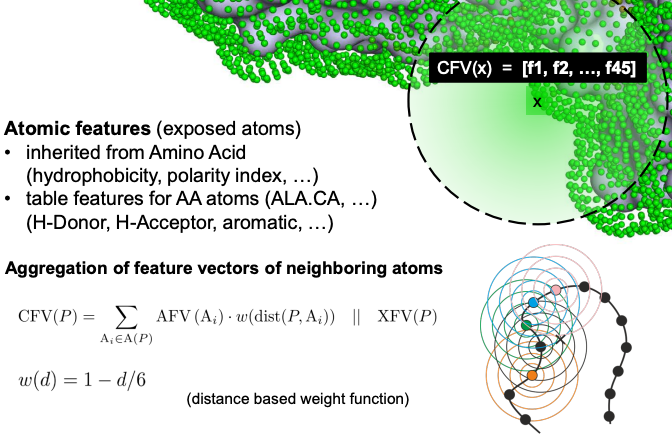
\includegraphics[width=1\textwidth]{img/slide_p2rank.png}\\
            \source{Radoslav Krivák and David Hoksza}
            \label{fig:p2rank}
            \end{minipage}
        \end{figure}
    \item \textbf{Ligandability Prediction}: A Random Forest classifier is used to predict the ligandability score for each Connolly point, indicating the likelihood that a point is part of a ligand-binding site.
    \item \textbf{Clustering}: Connolly points with high ligandability scores are clustered using a single-linkage clustering method, representing potential binding pockets on the protein surface.
    \item \textbf{Ranking}: Each predicted pocket is assigned a score based on the cumulative ligandability scores of its constituent points, helping prioritize the most likely binding sites for further analysis or docking studies.
\end{enumerate}

P2Rank's approach can significantly enhance the accuracy of predicting enzyme-mediated degradation of pesticides by providing detailed insights into the binding interactions at the molecular level. This integration of deep learning and enzyme analysis forms a robust framework for developing bioremediation strategies and understanding the environmental fate of various pollutants. \autocite{krivakP2RankMachineLearning2018}

\subsection{Introduction to Recurrent Neural Networks}
\label{sec:Introduction to Recurrent Neural Networks}

Recurrent Neural Networks (RNNs) are a class of artificial neural networks designed to recognize patterns in sequences of data such as text, genomes, handwriting, and spoken words. Unlike traditional feedforward neural networks, RNNs have connections that form directed cycles, allowing information to persist. This makes them particularly powerful for tasks that involve sequential data, where the order of the data points matters.

Recurrent Neural Networks (RNNs) are designed to process sequences of data by maintaining a memory of previous inputs. This memory allows RNNs to make use of information from earlier in the sequence to influence the current processing step, which is essential for understanding context in sequential data. The fundamental difference between RNNs and traditional neural networks is the presence of loops in the network that enable the persistence of information across time steps.

Recurrent Neural Networks (RNNs) are designed to process sequences of data by maintaining a memory of previous inputs. This memory allows RNNs to make use of information from earlier in the sequence to influence the current processing step, which is essential for understanding context in sequential data. The fundamental difference between RNNs and traditional neural networks is the presence of loops in the network that enable the persistence of information across time steps.

The basic structure of an RNN includes an input layer, a hidden layer with recurrent connections, and an output layer. At each time step, the hidden layer receives the input data and its own previous state, allowing it to retain and process information from previous steps in the sequence.

One of the key advancements in RNNs is the development of Long Short-Term Memory (LSTM) networks and Gated Recurrent Units (GRUs), which are designed to overcome the limitations of traditional RNNs, such as the vanishing gradient problem. These architectures use gating mechanisms to control the flow of information, making it easier to capture long-term dependencies in data.

In the context of bioinformatics, RNNs, particularly LSTMs and GRUs, are extensively used for sequence analysis tasks such as protein secondary structure prediction, gene expression analysis, and more. They are effective because they can handle the sequential nature of biological data and capture dependencies that span over long sequences. LSTM networks are a type of RNN that can learn long-term dependencies. They incorporate memory cells that can maintain their state over long periods. LSTMs have three main gates (input gate, forget gate, and output gate) that regulate the flow of information into and out of the memory cell, thus enabling the network to remember important information for longer durations. \autocite{hochreiterLongShortTermMemory1997}

The following image illustrates the basic structure of an RNN:

\begin{figure}[hbt]
    \centering
    \begin{minipage}[t]{\textwidth}
    \caption{A diagram for a one-unit recurrent neural network (RNN).}
    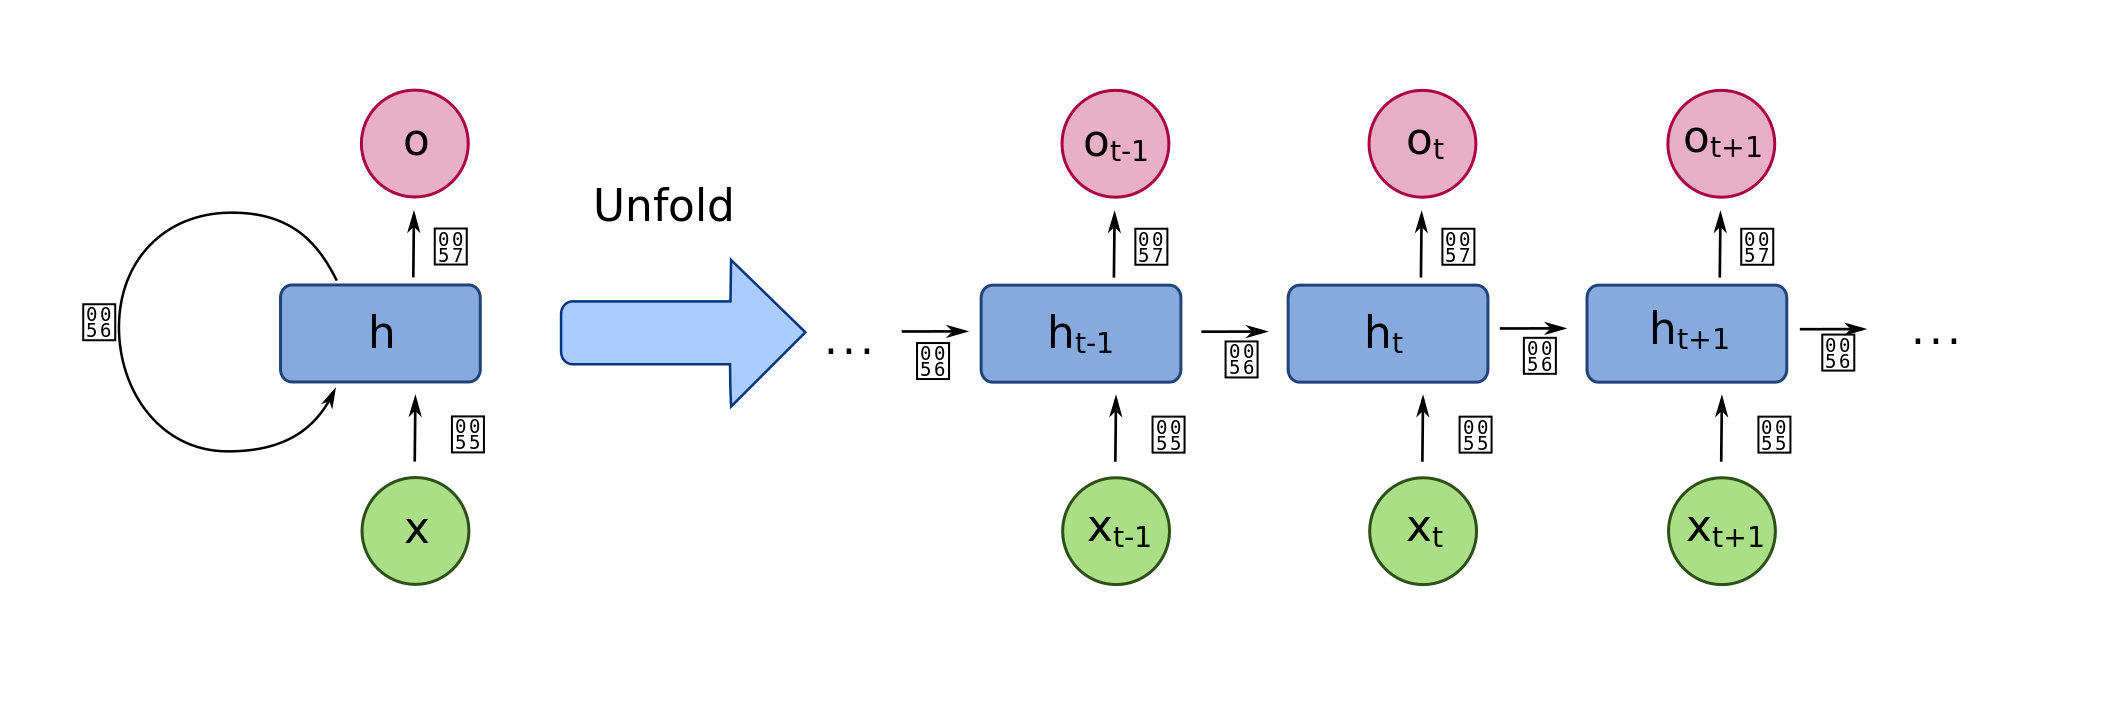
\includegraphics[width=1\textwidth]{img/Recurrent Neural Network Unfold.png}\\
    \source{fdeloche, CC BY-SA 4.0 via Wikimedia Commons}
    \label{fig:RNN}
    \end{minipage}
\end{figure}

\begin{enumerate}
    \item Input Sequence (x): The green circles represent the input data at different time steps ($ x_{t-1}, x_{t}, x_{t+1} $).
    \item Hidden State (h): The blue rectangles represent the hidden state of the network. At each time step, the hidden state (h) is updated based on the current input and the previous hidden state ($h_{t-1}, h_{t}, h_{t+1}$).
    \item Output Sequence (o): The pink circles represent the output of the network at each time step ($o_{t-1}, o_{t}, o_{t+1}$).
\end{enumerate}

The recurrent connection (arrow looping back) in the hidden state allows information to persist across time steps, enabling the network to maintain context and capture dependencies in the sequence data.

In this study, RNNs are employed for predicting the enzyme class based on the amino acid sequences of a ligand binding site. The sequential nature of the amino acid sequences makes RNNs well-suited for this task, as they can capture the dependencies and patterns in the data that are crucial for predicting enzyme classes accurately. Especially for complex and long sequences, RNNs, particularly LSTMs, are effective in learning the underlying structure and relationships in the data.

\subsection{Evaluation of Deep Learning Models}
\label{sec:Evaluation of Deep Learning Models}

Evaluating deep learning models involves several metrics and techniques to ensure their accuracy and generalizability. This is essential not only for validating the model’s performance but also for comparing it against other models. Using independent datasets for benchmarking is crucial to demonstrate the model's robustness and applicability to real-world scenarios. Several key metrics are commonly used to evaluate deep learning models:

\begin{enumerate}
    \item \textbf{Accuracy:} The ratio of correctly predicted instances to the total instances. It provides a straightforward measure of performance but can be misleading if the data is imbalanced. \autocite{AccuracyPrecision2024}
    \item \textbf{Precision:} The ratio of true positive predictions to the total predicted positives. Precision is crucial when the cost of false positives is high.
    \item \textbf{Recall (Sensitivity):} The ratio of true positive predictions to the total actual positives. Recall is important when the cost of false negatives is high. \autocite{PrecisionRecall2024}
    \item \textbf{F1-Score:} The harmonic mean of precision and recall, providing a single metric that balances both. It is useful when there is an uneven class distribution. \autocite{Fscore2024}
    \item \textbf{ROC-AUC (Receiver Operating Characteristic - Area Under Curve):} A performance measurement for classification problems at various threshold settings. It tells how much the model is capable of distinguishing between classes. The image shows an example of an ROC-AUC curve. As the curve gets closer to the top-left corner, the model's performance improves. \autocite{ReceiverOperatingCharacteristic2024}
    \begin{figure}[hbt]
        \centering
        \begin{minipage}[t]{.6\textwidth}
        \caption{AUC - ROC Curve}
        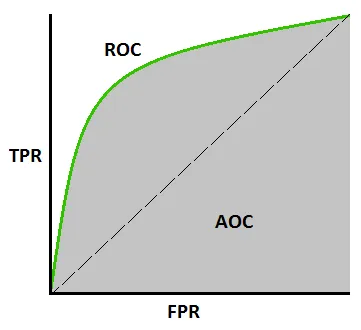
\includegraphics[width=1\textwidth]{img/ROC_AUC.png}\\
        \source{Sarang Narkhede via towardsdatascience.com}
        \label{fig:AUC-ROC}
        \end{minipage}
    \end{figure}
\end{enumerate}

Using these metrics, the performance of deep learning models can be tested on independent datasets. This is critical for ensuring that the models are not just overfitting to the training data but can generalize well to new, unseen data. By applying the models to benchmark datasets, researches can objectively measure and compare their performance. For instance, in the case of predicting enzyme-mediated pesticide degradation, using independent datasets ensures that the model’s predictions are reliable and can be generalized across various enzyme and pesticide types.